\documentclass{beamer} 

\usepackage[utf8]{inputenc}
\usepackage[T1]{fontenc}
\usepackage{graphicx}
\usepackage[serbian]{babel}
\usepackage{multicol}
\usepackage{tikz}
\usetikzlibrary{shapes.geometric, arrows}


\usetheme{Berlin}
\begin{document}


% TikZ blok dijagram stilovi
\tikzstyle{block} = [rectangle, rounded corners, minimum width=3cm, minimum height=1cm, text centered, draw=black, fill=blue!30]
\tikzstyle{arrow} = [thick,->,>=stealth]

\title{VertexVoyage: Distribuirani node2vec algoritam za embedovanje čvorova u realnim mrežama}
\author{Stefan Nožinić \\
Departman za matematiku i informatiku \\
Prirodno-matematički fakultet \\
Univerzitet u Novom Sadu. \\
Tip rada: master rad \\
Mentor: \MakeLowercase{dr} Miloš Savić
}

\frame{
\titlepage
}

\section{Uvod i Motivacija}
\begin{frame}{Uvod}
    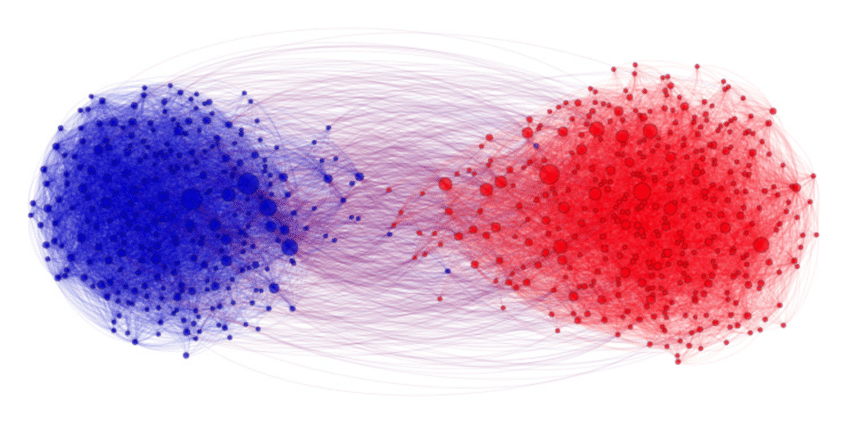
\includegraphics[width=\textwidth]{png/uvod.png}
    % add footnote
    \begin{footnotesize}
        Izvor: Interian, Ruben i Ribeiro, Celso. (2018). An empirical investigation of network polarization. Applied Mathematics and Computation. 339. 651-662. 10.1016/j.amc.2018.07.066.
    \end{footnotesize}
\end{frame}

\begin{frame}
	\frametitle{Ugrađivanje čvorova}
	Neka je $ G = (V, E) $ graf, tada je ugrađivanje funkcija 

	$$ U : V \to \mathbb{R}^n $$ 

	koja preslikava čvorove grafa u n-dimenzionalni euklidski prostor tako da čvorovi koji su dosta međusobno povezani budu blizu po euklidskom rastojanju
	

\end{frame}

\begin{frame}{node2vec}
	\centering
    \begin{tikzpicture}[node distance=2cm]

    % Blokovi
    \node (walks) [block] {Slučajne šetnje po čvorovima grafa};
    \node (embedding) [block, below of=walks] {Ugrađivanje (Embedding)};

    % Strelice
    \draw [arrow] (walks) -- (embedding);

    \end{tikzpicture}
\end{frame}

\begin{frame}{3 pitanja u radu}
    \centering 
	\begin{tikzpicture}[node distance=2cm]
		\node (q1) [block, text width=8cm, align=center] {Koliko paralelni algoritam ubrzava ceo proces?};
		\node (q2) [block, text width=8cm, align=center, below of=q1] {Kako paralelizacija utiče na kvalitet rekonstrukcije grafa iz ugrađivanja?};		
		\node (q3) [block, text width=8cm, align=center, below of=q2] {Koliko je klasterovanje iz ugrađivanja serijskom implementacijom slično sa klasterovanjem i ugrađivanja paralelnom implementacijom};
	\end{tikzpicture}
\end{frame}


\section{Arhitektura}
\begin{frame}{Arhitektura}
    \centering
    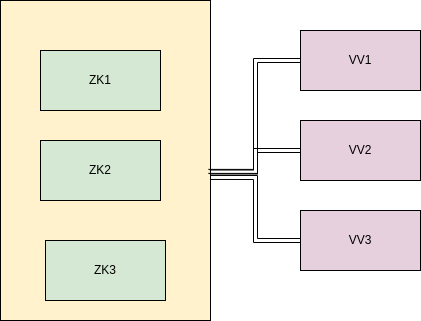
\includegraphics[height=0.8\textheight]{./png/Arhitektura i infrastruktura.drawio.png}
\end{frame}

\section{Blokovski prikaz algoritma}
\begin{frame}{Generalni Algoritam}
    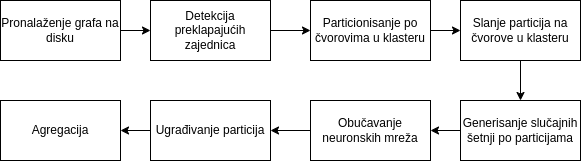
\includegraphics[width=\textwidth]{./png/Blokovski prikaz algoritma.drawio.png}
\end{frame}

\section{Particionisanje}
\begin{frame}{LFM Algoritam}
    \begin{itemize}
        \item Algoritam za detekciju preklapajućih zajednica 
        \item Za svaki čvor koji nije dodeljen zajednici, dodeljuje se nova zajednica 
        \item U zajednicu se dodaju susedni čvorovi čvorova u zajednici takvi da poboljšavaju kvalitet zajednice po funkciji $ f = \frac{k_\text{in}}{(k_\text{out} + k_\text{in})^\alpha} $ 
        \item Nakon dodavanja, čvorovi takvi da njihovo uklanjanje povećava kvalitet zajednice se uklanjaju
        \item Postupak se ponavlja sve dok postoje čvorovi koji nisu dodeljeni nekog zajednici
    \end{itemize}
\end{frame}

\begin{frame}{Modifikacija Algoritma}
    \begin{itemize}
        \item Zbog povećanja brzine, algoritam se modifikuje tako da ne traje sve dok postoje čvorovi koji nisu dodeljeni zajednici
        \item Umesto toga, algoritam se izvršava dok određeni broj čvorova nije dodeljen zajednici
    \end{itemize}
\end{frame}

\begin{frame}{Bin Packing}
    \begin{itemize}
        \item Nakon detekcije zajednica, potrebno je raspodeliti zajednice po čvorovima u klasteru
        \item U ovom radu, koristi se bin packing algoritam
        \item Algoritam raspoređuje zajednice po čvorovima tako da čvorovi u klasteru budu što sličniji po svom opterećenju
        \item Opterećenje čvora K kom su raspoređene zajednice $ S_K $ je $ \sum_{s \in S_K} |s| $
        \item Težine se zatim sortiraju u opadajućem redosledu, počevši od najveće.
        \item Inicijalno, maksimalna veličina (kapacitet) particije je prosečna veličina zajednice 
    \end{itemize}
\end{frame}

\begin{frame}
    \frametitle{Bin packing}
    \begin{itemize}
        \item Algoritam dodeljuje particije zajednicama, počevši od najveće zajednice. Uvek se dodeljuje particija koja je najmanje opterećena
        \item Ukoliko ne postoji particija koja ima potreban kapacitet, kapacitet particija se povećava za prosečnu veličinu zajednice koja još nije dodeljena particiji. 
        \item Ovaj proces se ponavlja dok sve zajednice ne budu raspoređene.
    \end{itemize}
\end{frame}


\section{Gubici strukturnih informacija}
\begin{frame}{Mera gubitka strukturnih informacija}
    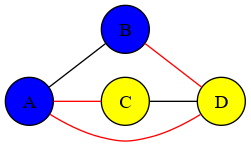
\includegraphics[width=\textwidth]{dot/graf.png}
\end{frame}

\begin{frame}{Mera gubitka strukturnih informacija}
    Neka je $ E_p $ skup svih grana koje sadrže čvorove takve da su oba čvora u particiji $ p $  i neka je $ P $ skup svih particija za graf $ G = (V, E) $

    Tada je mera gubitka strukturnih informacija $ L $ definisana kao

    $$ L = \frac{\sum_{p \in P} |E_p|}{|E|} $$

    Gde je $ |E_p| $ broj grana koje sadrže čvorove iz particije $ p $, a $ |E| $ ukupan broj grana u grafu $ G $
\end{frame}

\section{Rekonstrukcija}
\begin{frame}{Rekonstrukcija}
    $$ \text{recall} = \frac{\sum_{n \in V} \frac{|N(n) \cap N'(n)|}{|N(n)|}}{|V|} $$
    $$ \text{precision} = \frac{\sum_{n \in V} \frac{|N(n) \cap N'(n)|}{|N'(n)|}}{|V'|} $$
    $$ F_1 = \frac{2 \cdot \text{precision} \cdot \text{recall}}{\text{precision} + \text{recall}} $$
\end{frame}


\section{ARI}
\begin{frame}{Adjusted Rand Index (ARI)}
    \begin{itemize}
        \item Meri sličnost između dve klasterovanja
        \item Vrednost je bliska 0 za slučajno klasterovanje, a 1 za identična klasterovanja
        \item $ \text{ARI} = \frac{\text{RI} - \text{Expected\_RI}}{\text{max(RI)} - \text{Expected\_RI}} $
    \end{itemize}
\end{frame}

\section{Skupovi Podataka}
\begin{frame}{Skupovi Podataka}
    \begin{itemize}
        \item Poznati grafovi iz literature 
        \item Twitch mreža
        \item Sintetički grafovi 
    \end{itemize}
\end{frame}

\begin{frame}{Twitch}
    \centering
    \begin{tabular}{|c|c|c|c|c|}
        \hline
        \textbf{Karakteristika} & \textbf{Vrednost} \\
        \hline
        Broj čvorova & 168.114 \\
        Broj grana & 6.797.557 \\
        Gustina & 0.0005 \\
        \hline
    \end{tabular}
\end{frame}

\section{Rezultati}
\begin{frame}{Vreme particionisanja za neke popularne mreže}
    \centering
    \begin{table}
        \label{tab:4.2}
        \begin{tabular}{lp{1in}p{1in}p{0.5in}}
        Mreža & Vreme particionisanja & Broj čvorova & Broj grana \\
        \hline
        Zaharijev karate klub & 0.001 & 34 & 78 \\
        Les Mis & 0.004 & 77 & 254 \\
        Davis southern women & 0.004 & 32 & 89 \\
        Florentine families & 0.0006 & 15 & 20 \\
        Twitch  & 1638.00 & 168114 & 6797557 \\
    \end{tabular}
\end{table}
\end{frame}
    
\begin{frame}{Vreme particionisanja za sintetički graf}
    \centering
    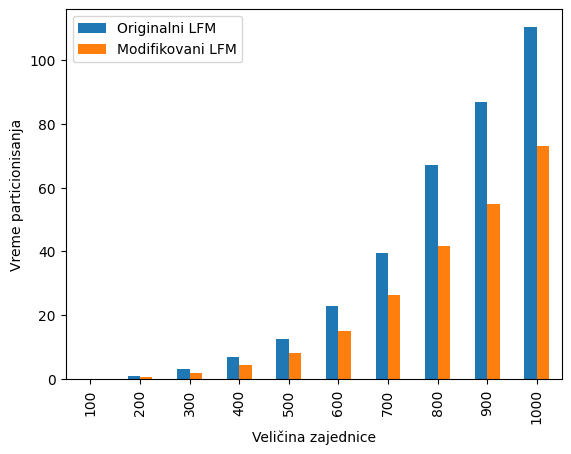
\includegraphics[height=0.8\textheight]{csv/4.3.png}
\end{frame}

\begin{frame}
    \frametitle{Ukupno vreme ugrađivanja na sintetičkom grafu}
    \centering
    \begin{table}
        \label{tab:4.13}
        \begin{tabular}{p{1in}p{1in}p{1in}}
            \hline
            Broj šetnji & Vreme (serijska implementacija) & Vreme (paralelna implementacija) \\
            \hline
        300 & 27.032333 & 46.671196 \\
        600 & 34.207081 & 52.855629 \\
        900 & 49.972453 & 59.757545 \\
        1200 & 61.620000 & 68.144959 \\
        1500 & 72.930000 & 77.180386 \\
        1800 & 85.400000 & 84.556964 \\
        2100 & 97.770000 & 93.268643 \\
        2400 & 109.315041 & 100.895541 \\
        \hline
    \end{tabular}
\end{table}
\end{frame}

\begin{frame}
    \frametitle{Specifikacija sintetičkog grafa koji je rekonstruisan iz ugrađivanja}
    \begin{itemize}
        \item Broj čvorova po zajednici: 1000
        \item Broj zajednica: 2
        \item Verovatnoća povezivanja čvorova unutar zajednice: 0.1
        \item Verovatnoća povezivanja čvorova između zajednica: 0.01
    \end{itemize}
\end{frame}

\begin{frame}{F1 mera rekonstrukcije sintetičkog grafa}
    \centering
        \begin{table}
        \label{tab:4.10}
        \begin{tabular}{p{1in}p{1in}p{1in}}
        \hline
        Broj šetnji & F1 mera serijske implementacije & F1 mera paralelne implementacije \\
        \hline
        100 & 0.058427 & 0.108415 \\
        200 & 0.074563 & 0.120501 \\
        300 & 0.105385 & 0.136140 \\
        400 & 0.121520 & 0.149141 \\
        500 & 0.118749 & 0.156055 \\
        600 & 0.117749 & 0.171991 \\
        700 & 0.119408 & 0.173323 \\
        800 & 0.121913 & 0.172578 \\
        900 & 0.129534 & 0.180858 \\
        \hline
    \end{tabular}
    \end{table}
\end{frame}
    
\begin{frame}{F1 mera rekonstrukcije Zaharijevog karate kluba}
    \centering 
    \begin{table}
        \label{tab:4.4}
        \begin{tabular}{p{1in}p{1in}p{1in}}
        \hline
        Broj šetnji & F1 mera serijske implementacije & F1 mera paralelne implementacije \\
        \hline
        100 & 0.580310 & 0.575914 \\
        200 & 0.624504 & 0.654000 \\
        300 & 0.701834 & 0.645231 \\
        400 & 0.717563 & 0.708462 \\
        500 & 0.727480 & 0.711250 \\
        600 & 0.774543 & 0.725454 \\
        700 & 0.786713 & 0.744720 \\
        800 & 0.787490 & 0.721272 \\
        900 & 0.775203 & 0.717695 \\
        \hline
    \end{tabular}
\end{table}
\end{frame}

\begin{frame}{Sličnost klasterovanja}
    \centering
    \begin{table}
        \label{tab:4.11}
        \begin{tabular}{p{1in}p{1in}}
        \hline
        Skup podataka & Sličnost \\
        \hline
        Zaharijev karate klub & 1.000000 \\
        Davis Southern Women & 0.650000 \\
        Florentine Families & 0.380000 \\
        Les Miserables & 0.450000 \\
        Twitch & 0.970000 \\
        SBM generisan graf & 0.990000 \\
        \hline
    \end{tabular}
    \end{table}
\end{frame}

\begin{frame}{Parametri modela}
    \centering
    \begin{table}
        \label{tab:4.12}
        \begin{tabular}{p{2in}p{2in}}
        \hline
        Parametar & Vrednost \\
        \hline
        Veličina šetnje (walk\_size) & 800 \\
        Dimenzija (dim) & 128 \\
        Veličina prozora (window\_size) & 10 \\
        Broj epoha (epochs) & 10 \\
        Parametar p & 0.250000 \\
        Parametar q & 4.000000 \\
        Broj negativnih uzoraka (negative\_sample\_num) & 10 \\
        Stopa učenja (learning\_rate) & 0.010000 \\
        Broj šetnji & 400 \\
        \hline
    \end{tabular}
\end{table}
\end{frame}


\begin{frame}{Odnos F1 mera u zavisnosti od gubitaka strukturnih informacija}
    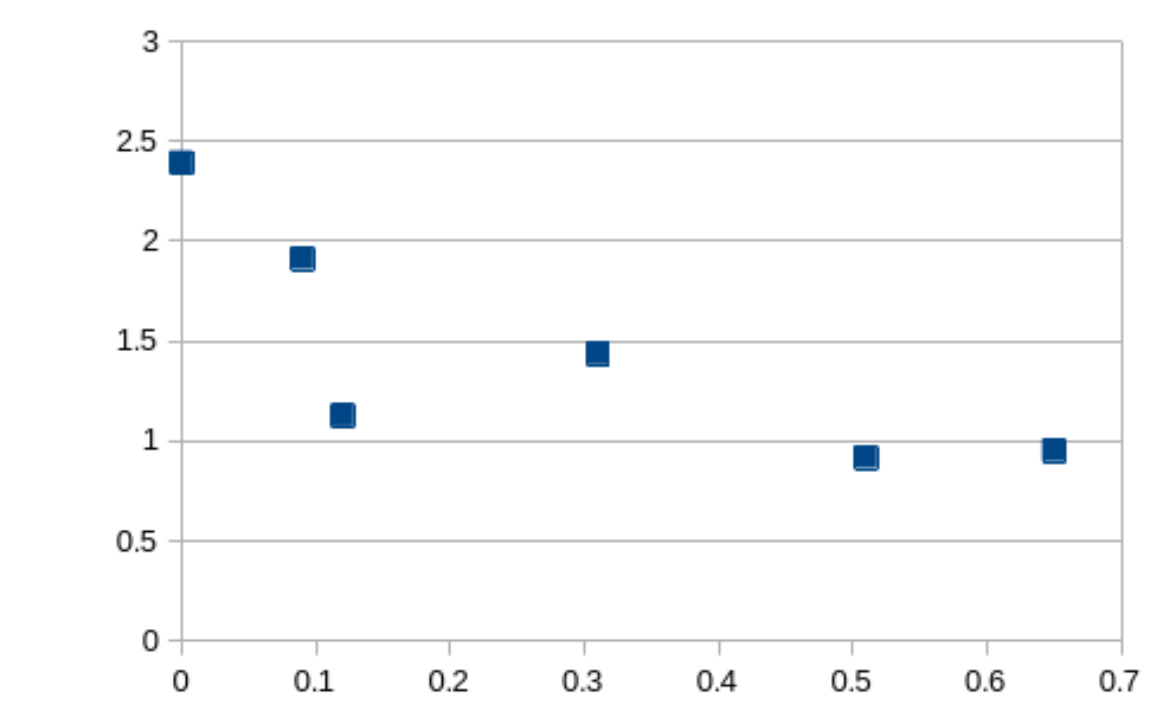
\includegraphics[height=0.8\textheight]{png/grafik.png}
\end{frame}

\section{Zaključak}
\begin{frame}{Zaključak}
    \begin{itemize}
        \item Rezultati su pokazali da je paralelna implementacija algoritma brža od serijske, nakon određenog broja šetnji, dok zadržava kvalitet rekonstrukcije grafa
        \item Rezultati su pokazali da je klasterovanje dobijeno paralelnim ugrađivanjem slično klasterovanju dobijenom serijskim ugrađivanjem
        \item Unapređenja:
        \begin{itemize}
            \item Upotreba specifične baze podataka koja bi indeksirala čvorove tako da particionisanje bude brže
            \item Poređenje paralelne i serijske implementacije na drugim primenama
            \item fino podešavanje parametara modela za velike mreže 
        \end{itemize}
    \end{itemize}
\end{frame}



\begin{frame}
	\frametitle{Pitanja}
	\begin{center}
		\huge{?}
	\end{center}
\end{frame}


\end{document}
